\section{Zielsetzung}
\label{sec:Zielsetzung}

Es soll anhand des Photoeffekts der Zusammenhang zwischen der Wellenlänge des Lichts und der Maximalenergie
der emittierten Elektronen, sowie die Abhängigkeit des Elektronenstroms von der an der Photozelle angelegten
Spannung untersucht werden.

\section{Theorie}
\label{sec:Theorie}

Beim Photoeffekt (lichtelektrischer Effekt) werden Elektronen
aus einer Metalloberfläche durch Bestrahlung mit Licht gelöst.

\subsection{Licht als Welle und Teilchen}

Licht besitzt sowohl Licht- als auch Welleneigenschaften. Diese
beiden Eigenschaften können durch Experimente separat nachgewiesen
werden. Beim Compton-Effekt lässt sich die korpusulare Natur
nachweisen, während bei der Interferenz der Wellencharakter zum
beobachten ist.\\
Die beiden Theorien lassen sich nicht miteinander vereinen. Dies geht 
allein schon aus der unterschiedlichen mathematischen Beschreibung
der Phänomene hervor. Während die Teilcheneigenschaften sich
mit der Newtonschen Punktmechanik beschreiben lassen, wird der
Wellencharakter anhand der Maxwellschen Gleichungen (Wellengleichung)
beschrieben.\\
Durch diese Inkonsistenz des Lichts, ist eine klassische 
Betrachtungsweise ausgeschlossen. Die Quantenelektrodynamik (QED)
liefert hier die Möglichkeit eine widerspruchsfreie Theorie
zu liefern. In dieser Theorie sind die Teilchen- Und Wellenzüge
des Lichts nämlich Grenzfälle.\\
Jeder Grenzfall lässt sich durch eine geeignete Formel beschreiben.
Die Vermischung ist eher kompliziert. Die jeweilige Annäherung
der Gleichung hängt vom Experiment ab.\\
Wenn über eine große Anzahl von Photonen gemittelt wird, wird
generell das Wellenmodell verwendet und bei einer Wechselwirkung
mit Materie das Teilchenmodell. \\

\subsection{Photoeffekt nach der einsteinschen Korpuskulartheorie}

Beim Experiment zum lichtelektrischen Effekt wird im Vakuum 
eine Festkörperoberfläche (vorzugsweise Metall) mit monochromatischen
Licht bestrahlt. Diese Oberfläche ist die Photokathode. Ihr gegenüber
ist eine Auffängerelektrode gestellt, welche ein positives Potential
in Bezug auf die Photokathode besitzt. Die beiden Metallplatten
sind über ein Strommessgerät miteinander verbunden.\\
Wenn sich Elektronen aus der Photokathode lösen, werden sie in Richtung
Auffängerelektrode beschleunigt und erzeugen beim Aufprall einen Stromfluss
der gemessen wird.\\
Durch diesen Aufbau lassen sich diese Erkenntnisse ziehen:
\begin{itemize}
    \item Die Anzahl der gelösten Elektronen pro Zeit ist proportional zur Lichtinsensität.
    \item Die Energie der Photoelektronen ist proportional zur Lichtfrequenz, aber nicht zur Lichtinsensität.
    \item Es gibt eine untere Grenzfrequenz, wo der Photoeffekt nicht zu beobachten ist.
\end{itemize}

Diese Ergebnisse sind nicht mittels des Wellenmodells erklärbar. 
Beim Wellenmodell könnte man das Loslösen der Elektronen dadurch
erklären, dass die Elektronen durch das E-Feld in Schwingung versetzt
werden und die Festkörperoberfläche verlassen, sobald die Schwingungsamplitude
zu groß wird. Dies würde jedoch auch bedeuten, dass Elektronen sich
bei großer Wellenlänge und Intensität ebenfalls loslösen würden. Zudem
sollte es eine bestimmte Frequenz geben, bei der Resonanzphänomene zu beobachten
sind, wo der Photoeffekt bevorzugt auftritt. Auch müsste die Elektronenenergie
mit der Lichtinsensität steigen.\\
Eben das lässt sich alles nicht beobachten.\\
Nimmt man nun aber an, dass die Energie in Volumina subatomarer
Größe konzentriert sind, lassen sich die Erkenntnisse des Experiments
erklären. Diese Lichtquanten (Photonen) haben praktisch eine verschwindende
Ausdehnung.\\
Nach Einstein sind diese Korpuskel identisch mit Planckschen Energiequanten.\\
Mit den Planckschen Energiequanten lassen sich folgende Annahmen postulieren:
\begin{itemize}
    \item monochromatisches Licht mit einer Frequenz $f$ besteht aus Photonen. Diese bewegen sich geradlinig mit $c$ und haben jeweils die Energie $hf$ (mit $h=$ Plancksches Wirkungsquantum)
    \item Wenn ein Photon seine Energie auf ein Elektron überträgt, teilt sich diese in die Austrittsarbeit $A_k$ 
    (Energie die benötigt wird, damit sich Elektronen von der Festkörperoberfläche lösen können) und die kinetische Energie des Photons.
\end{itemize}
Mit der Energieerhaltung ergibt sich also
\begin{align}
\label{eqn:Energiebilanz}
    hf = E_{kin} + A_k.
\end{align}
Aus diesen beiden Annahmen folgt also, dass wenn 
\begin{align}
\label{eqn:hf_kleiner}
    hf < A_k
\end{align}
ist, kein Photoeffekt
mehr zu beobachten ist. Das lässt sich auch im Experiment beobachten.\\
Eine weitere Annahme ist,
\begin{itemize}
    \item dass die Lichtitensität proportional zur Zahl der Photonen 
pro Zeit- und Raumwinkeleinheit ist.
\end{itemize}
Durch diese Annahme lässt sich auch die erste Erkenntnis aus dem Experiment
erklären.\\

\subsection{Experimentelle Untersuchung des Photoeffekts}

Für die experimentelle Untersuchung wird eine Photozelle verwendet, 
ein evakuierter Glaskolben mit zwei Elektroden. Die Photokathode ist auf
ihrer Innenseite mit einer Metall- oder Legierungsschicht aufgedampft,
welche während des Experiments bestrahlt wird. Die Anode ist ein kreisförmiger Drahtring,
die wenige Millimeter Abstand zur Kathodenoberfläche hat.\\
Die Energie lässt sich mit der Gegenfeldmethode messen. Dazu legt man 
eine variable Spannung $U$ an, die abremsendes Feld für die Elektronen erzeugt.
Der gemessene Strom zwischen den Elektroden verschwindet nun spätestens dann,
wenn 
\begin{align}
    \label{eqn:StromWeg}
    e_0 U_g = \frac{1}{2} m_0 v^2_{max}
\end{align}
ist. $v_{max}$ ist die Geschwindigkeit der schnellsten Elektronen, $m_0$ die Ruhemasse
des Elektrons, $e_0$ die Elementarladung und $U_g$ die Gegenspannung.\\
Für die schnellsten Elektronen gilt zudem nach \autoref{Energiebilanz} und 
\autoref{StromWeg} folgende Relation:
\begin{align}
    \label{eqn:1und2}
    hf = e_0 U_g + A_k.
\end{align}
Durch diese FOrmel sollte sich dann das Verhältnis von Wirkungsquantum $h$ zur
Elementarladung $e_0$ bestimmen lassen. Beim Experiment selbst lässt sich jedoch 
feststellen, dass der Photostrom nicht schlagartig bei $U = U_g$ verschwindet, sondern 
bereits bei $U < U_g$ deutlich sinkt. Die Strom-Spannungskurve hat also
die in (Foto einfügen) gezeigte Form.\\
\begin{figure}
        \centering
        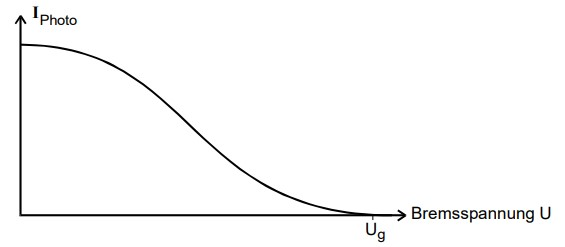
\includegraphics{Bilder/PhotoStrom1.jpg}
        \caption{Photostrom in Abhängigkeit von Bremsspannung einer Photozelle bei monochromatischen Licht.\cite{sample}}
        \label{fig:Reflexion}
\end{figure}
Dadurch wird die Bestimmung von $U_g$ erschwert. Das Problem kommt dadurch zur Stande,
dass die Photoelektronen eine Energieverteilung besitzen. Die Energie hängt hier davon ab,
wie viel Energie sie im Festkörper vorher besessen haben.\\
Über diese Energieverteilung macht die Fermi-Dirac-Statistik eine Aussage. 
Diese besagt, dass sich die Energie der Valenzelektronenvon 0 bis zur Fermi-Energie
erstrecken.\\
Man kann zeigen, dass unter bestimmten Voraussetzung der parabolische Zusammenhang
\begin{align*}
    I_{Ph} \~{} U^2
\end{align*}
besteht. Mit diesem Zusammenhang kann man $U_g$ erhalten, indem man $\sqrt{I}$ gegen
$U$ aufträgt und $U_g$ als Schnittpunkt mit der $U$-Achse entnimmt.\\
Bei der verwendeten Apparatur verwendet man falsche Ergebnisse, da nicht alle Photoelektroden
die Anode erreichen, da ihre Oberfläche zu klein ist. Eine weitere Voraussetzung unter der
nicht alle Photoelektronen die Anode erreichen ist, wenn das Anodenmaterial eine zu hohe
Austrittsarbeit $A_A$ hat. Wenn man zwei Metalle miteinander verbindet, stellen sich ihre
Fermi-Niveaus auf gleiche Höhe ein. Es tritt also auch kein Photostrom auf (trotz $hf > A_k$), wenn $hf < A_A$
ist, da die ELektronen dann gegen ein Gegenfeld anlaufen müssten.\\
Es tritt also dann ein Photostrom auf, wenn
\begin{align}
    \label{eqn:Aa}
    hf + e_0 U_b \geq A_A
\end{align}
gegeben ist. Hierbei ist $U_b$ eine Beschleunigungsspannung, die gegen das Gegenfeld
wirkt.\\
Bei dem später aufgeführten Experiment kann man sogar einen negativen
Strom beobachten, wenn $U_b$ hoch genug ist. Das erschwert ebenfalls die Bestimmung von $U_g$,
da sich der Strom mit dem Photostrom überlagert.\\
\begin{figure}
    \centering
    \includegraphics{Bilder/Potentialverhältnisse.jpg}
    \caption{Abb. links: Potentialverhältnisse zwischen Anode und Kathode unter Berücksichtigung der Austrittsarbeiten
    von Anode und Kathode. Abb. rechts: Anlegen eines beschleunigenden Potentials $U_b$ zur Erzeugung eins Photostroms. \cite{sample}}
    \label{fig:Reflexion}
\end{figure}

\newpage